\chapter{Aufgabe 1}

\section{a)}
\textit{Skizzieren Sie den internen Aufbau einer kontaktbehafteten Chipkarte und charakterisieren Sie die einzelnen Komponenten.}\\

\noindent
Die Skizze einer kontaktbehafteten Chipkarte ist in Abbildung~\ref{fig:chipkarte} angegeben.
Es erfolgt eine allgemeine Beschreibung von Chipkarten und der darin verwendeten Komponenten:

\begin{itemize}
    \itemsep0.5em
    \item Chipkarten gibt es in unterschiedlichen Bauformen, die über ISO 7810 standardisiert sind.
    Die Chips selber sind in einen Kartenkörper eingefasst, der meist aus PVC (\textit{Polyvinylchlorid}) besteht.
    \textit{Schartner} stellt einige der o.a. Bauformen in~\cite[]{ITS5} vor, darunter \textit{ID-1}, \textit{ID-00}, \textit{ID-000}, \textit{Mini-UICC}, wobei dem Format und dem Einsatzzweck der Chipkarte nach weitere \textit{optische} Informationen auf der Karte selber untergebracht werden können, die bspw. zur Personalisierung der Karte und Identifikation des Kartenbesitzers dienen, darunter u.a. Namen/ID-Nummern (Bank-/Kreditkarte), \textit{Profilfoto} des Besitzers, schwer zu fälschende Muster und Zeichen (\textit{Hologramme}, \textit{Guillochen}, vgl.~\cite[74]{ITS5}).\\
    Erwähnenswert sind in diesem Zusammenhang \textit{Hybridkarten}, die neben einem Chip auch noch einen Magnetstreifen besitzen, um eine gewisse Kompatibilität zu anderen Lesegeräten herzustellen (\cite[4]{ITS5}).

    \item Der in den Kartenkörper eingefasste Chip besitzt unterschiedliche Segmente, die bestimmte Funktionalitäten realisieren.
    Diese werden im Folgenden kurz beschrieben:
    \begin{itemize}
        \item Ohne auf Details einzugehen, lässt sich die Architektur des Chips wie folgt beschreiben: Die CPU des Chips ist über einen Bus mit den verschiedenen \textit{Speichereinheiten} verbunden. Chipkarten, die die Sicherheitsziele \textit{Integrität}, \textit{Authentizität} und \textit{Vertraulichkeit} umsetzen, verteilen die Daten auf Speicherbereiche, die ein \textit{Lesen}, \textit{Löschen}, \textit{Ändern} unterschiedlich kombiniert erlauben: So ist der \textit{(P)ROM} dafür verantwortlich, das Betriebssystem unveränderlich zu speichern, \textit{EEPROM} dient als nichtflüchtiger Speicher, der (Sitzungs-)Daten speichern und wieder zur Verfügung stellen kann, und der \textit{RAM} dient auch hier - wie aus anderen Rechnerarchitekturen bekannt - als (flüchtiger) Arbeitsspeicher.

        \item Damit die Karte überhaupt in den Betriebsmodus übergehen kann, muss der Chip (die CPU) mit Spannung versorgt werden. Hierzu dient das in der Abbildung angegebene Segment \textbf{C1}.

        \item Sobald die CPU mit Energie versorgt wird, kann ein Terminal über das Segment \textbf{C2} einen ``Reset`` der Karte veranlassen, woraufhin die Kommunikationssitzung von der Karte über ein sogenanntes \textit{ATR} (\textit{Answer to Reset}) bestätigt werden kann.

        \item Zur \textit{seriellen} Kommunikation dient das Segment \textbf{C7} (\textit{Input} / \textit{Output}), wobei die Synchronisation zwischen Terminal und Karte über das Segment \textbf{C3} (\textit{CLK} - Clock, Takt) realisiert wird.
    \end{itemize}
\end{itemize}

\begin{figure}
    \centering
    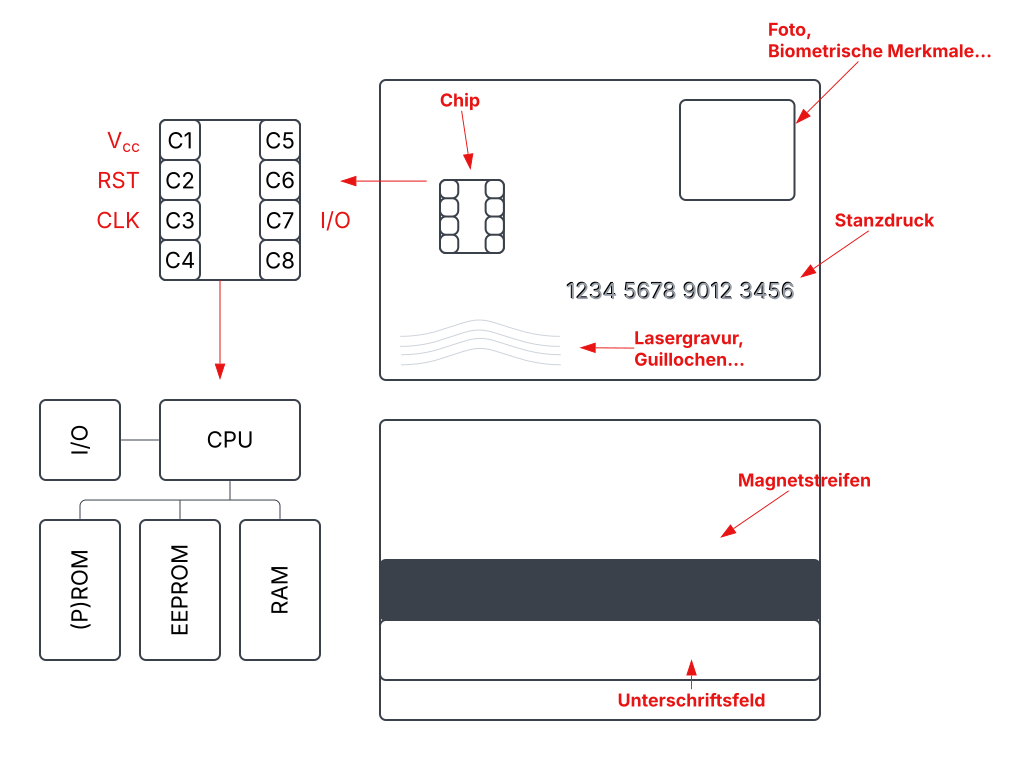
\includegraphics[scale=0.4]{aufgabe 1/img/chipkarte.svg}
    \caption{Skizzenhafte Darstellung einer kontaktbehafteten Chipkarte und möglicher Komponenten. (Quelle: in Anlehnung an~\cite[\textbf{Abb. 2.1}, 9 sowie \textbf{Abb. 2.2}, 10]{ITS5})}
    \label{fig:chipkarte}
\end{figure}


\section{b)}

\textit{Welche Komponenten werden für eine Dual‐Interface‐Chipkarte zusätzlich benötigt?}\\

\noindent
Als \textit{Dual-Interface-Chipkarten} (auch: \textit{Kombikarte},~\cite[4]{ITS5}) werden diejenigen Chipkarten bezeichnet, die sowohl \textit{kontaktlos} als auch \textit{kontaktbehaftet} mit einem Terminal kommunizieren können.\\
Da die Energieversorgung solcher Karten über \textit{elektromagnetische} oder \textit{kapazitive Kopplung} erfolgt, sind Schreib-/Lesedistanzen zwischen Terminal und Karte begrenzt (vgl.~\cite[27]{ITS5}).

\noindent
Damit bspw. kontaktlos nach ISO 14443\footnote{
    \url{https://en.wikipedia.org/wiki/ISO/IEC_14443}, abgerufen 15.04.2025
} kommuniziert werden kann, benötigt die Karte als \textit{physische Voraussetzung} eine Komponente zum Senden/Empfangen von Daten, was über ein in die Karte eingelassenes \textit{RFID}\footnote{
    \textit{Radio-Frequency Identification} (\cite[95 f.]{ITS5})
}-Modul/ eine \textit{RFID}-Antenne realisiert wird (vgl.~\cite[27]{ITS5}).

\noindent
\textit{Logisch} benötigt der Prozessor als zusätzliche Komponente ein Interface zur Verarbeitung und Umsetzung der Protokolle, die mit der Funktechnologie einhergehen, wie es bspw. der \textit{Infineon SLE 66CLX800PE}\footnote{
    s.a.~\url{https://www.electronicsdatasheets.com/manufacturers/infineon-technologies-ag/parts/sle-66clx800pe-ms}, abgerufen 15.04.2025
}  anbietet (vgl.~\cite[11]{ITS5}).